Within this chapter the general design of the system implementing the new process is described. First of al the general design is discussed, followed by a explanation about the used languages and frameworks. Finally, the rule set request is explained. 

\section{General Design}
Due to the fact that the system should be a web application, a modified \gls{mvc} is used to split up business logic and the user interface presentation. The system has the following components:

%\begin{table}[h!]
	\begin{longtable}{|p{4cm}|p{11cm}|} \hline
		\rowcolor{Gray}Component & Functionality \\ \hline
		View & Presents the result of the  business logic and triggers the user interaction.\\ \hline
		Controller & Handles the communication between view and service in such a way, that the other components do not need to know from each other. The controller process all transmitted actions from the view and request the service for the corresponding tasks. The returned information are prepared for the view and presented through the view to the user. \\ \hline
		Service & This component holds the business logic of the system and coordinates the interactions with the \frqq information\flqq components. \\ \hline
		Model & Inside the model the information are stored, which are exchanged between all components.\\ \hline
		\Gls{erp} Connector & It is responsible for the communication with the \gls{erp}. As information it has to provide information about documents, customer and the employee uploaded the document. \\ \hline
		Signing Tool Connector & At this component the signing process of a selected document is managed. Therefore, information about the signers are required and the document file. \\ \hline
		User Reader & This component handles user and employee data from the company. It is responsible for the login to the system and should stores all members of the company with their position. The required informations are name, position, phone number and mail address, because they are either needed to give information who had to sign a document together with the user based on the rule set and to pass the required signer information directly to the signing tool. \\ \hline
		Rules Reader & An important component is the rules reader, because it knows the signing guideline of the company. It provides for te system the information which company positions had to sign a document based on its type, value and the user initiate the signing process.\\ \hline
		\caption{Listing of Systems Components}
		\label{tab:listingSystemComponents}
	\end{longtable}
%	\centering
%	\caption{Listing of Systems Components}
%	\label{tab:listingSystemComponents}
%\end{table}

In figure \ref{fig:generalDesign} the communication between the components is visualized.
The most communication is done with and from the service component. 
------ToDo-------------

\begin{figure}[h!]
	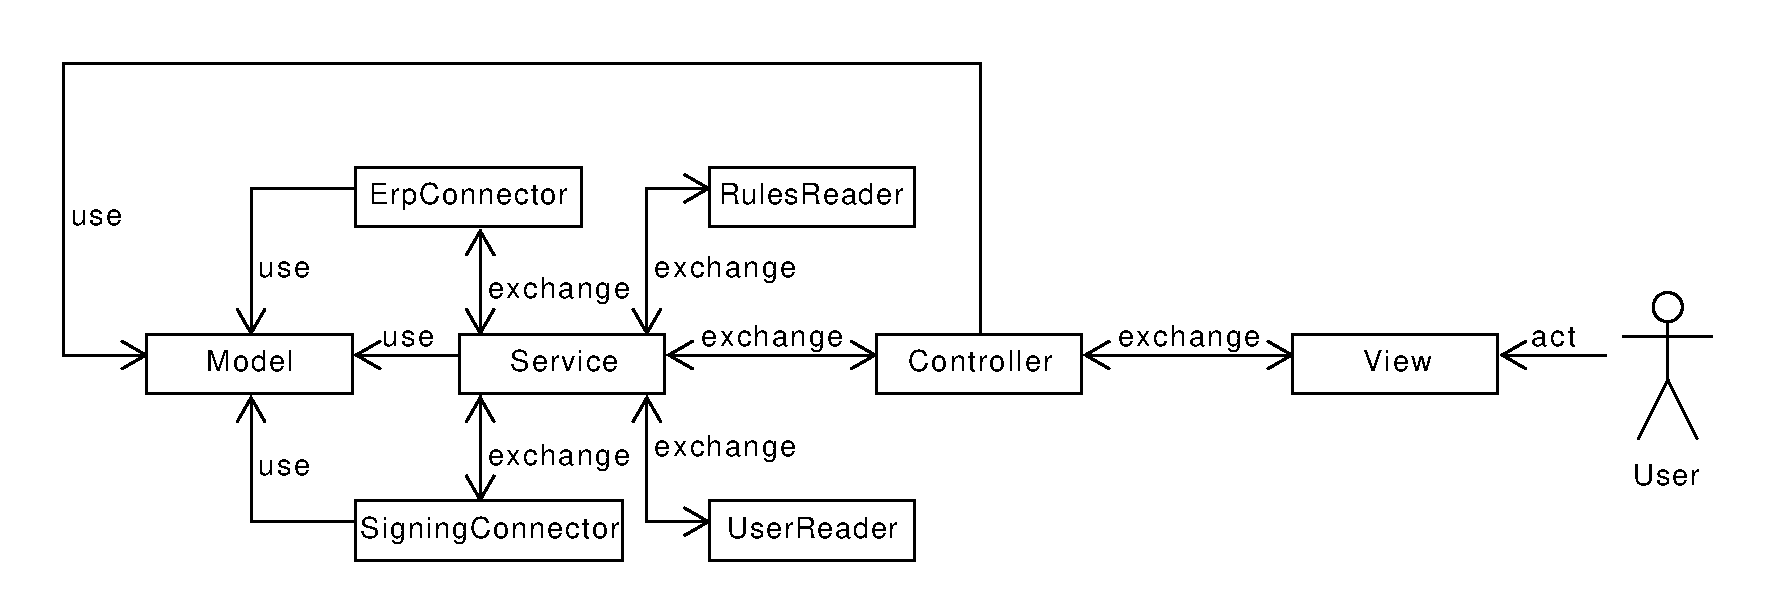
\includegraphics[width=\linewidth]{./design/images/generalCommunication.pdf}
	\centering
	\caption{General system design}
	\label{fig:generalDesign}
\end{figure}

Due to the fact that it is unclear which \gls{erp} will be used and that therefore no decision is made for a singing tool, the connector components should be variable as possible to be independent from the later tools. That leads to the design decision to define interfaces for those connectors, which are implemented with mocked systems to present the process. \newline
Beside of this interfaces two more should be created for the reader components, because those have connections the data storages, which depends company using the later system. In the most cases they have already a authentication system, that also stores the position of the company members. For the rules reader the preferences of the later administrators are important, because they are responsible to maintain the data and update them, if changes are made to the signing guideline. Therefore, it is important that they can choose a preferred system. In the following the interfaces are explained more in detail. The code is added in the appendix \ref{interfaceDef}.

\subsection*{Enterprise Resource Planning System Connector}
This interface defines the methods for the receiving information of documents from the \gls{erp}, the document file itself and the storing of the signed document. Important therefore is the search functionality. In general are a lot of documents stored inside an \gls{erp} and it is not possible to present them all in a lucid overview. At the moment it should be possible to search for the followings information of document: document type, document name, related customer name and the name of the employee, who created/stored the document inside the \gls{erp}.

\subsection*{Rule Reader}
Within this interface only one method is defined to get the information which combinations of company members have to right to sign the selected document. It will receive the information about the type of the document, the value of the document and the position of the user want to sign the document. The implementation follows always the request described in section \ref{sec:ruleRequest}.

\subsection*{Signing Tool Connector}
-----------------ToDo--------------------

\subsection*{User Reader}
Inside this interface different functionalities are defined, which are split up in the areas position groups and member information. In the first area the implementation provides the information which members have a certain position at the company. The second
area is responsible for giving specific information about a member. These information are company position, mail address and phone number.

\section{Used Programming Language and Frameworks}
- Spring Boot: easy set up, has already a lot of functionalities like security log in, embedded dbs / server, get new experiences, server configurations

At the start of the implementation a discussion were made, which programming language to use. Available were several options, because due to the usage of the framework \textit{DocuSign eSign} for mocking the signing tool. It provides different \glspl{sdk} like C\#, Node.js and Java \parencite{docusign2018sdk} and \gls{rest} \gls{api}. The choice was Java, because it is one of the standards programming languages of \gls{cc}, mostly well known by other programmers and it is the best known programming language of the author. Due to the fact that there are time issues at the end of the project, this language was selected.

Another decision was to use \textit{Maven}, because it builds the complete dependencies from the project independent from the \gls{os}. That is useful for automated testing in pipeline systems and deploying. \newline
Moreover, was the decision made to use \textit{Spring Boot}. With this tool it is simple to setup a project without installing server and databases to deploy. This is beneficial for prototyping, which should be made in this project. Furthermore, does the author not have experiences with the framework and an approach for the bachelor thesis is to get new experiences. Additional, provides \textit{Spring Boot} functionalities for security and \gls{mvc} applications, which are needed in the project. \newline
All other used tools and frameworks are listed in table \ref{tab:frameworks}.

\begin{table}[h!]
	\begin{tabular}{|p{2cm}|p{13cm}|} \hline
		\rowcolor{Gray}Framework/ Tool & Functionality \\ \hline
		Lombok & Project Lombok is an open source Java library that generates simple code (e.g. Getter and Setters) based on set annotations \parencite{lombok2018}.\\ \hline
		Mockito & Provides functionalities to mock classes and helps to test logic independent from the implementation \parencite{mockito2018}. \\ \hline
		H2 & This is a lightweight \gls{sql} \gls{db} with already existing \gls{api} for data transferring between system and \gls{db} \parencite{hs2018}. \\ \hline
		JUnit & This framework provides a lot of functionalities for testing like test suites or specific annotations for testing \parencite{junit2018}. \\ \hline
	\end{tabular}
	\centering
	\caption{List used Frameworks}
	\label{tab:frameworks}
\end{table}

\section{Rule Set Request}\label{sec:ruleRequest}
Inside the rule set the signing guideline is stored for the system. In general it can be said that there exist four general data sets:
\begin{itemize}
	\item Company positions: \newline
	Inside this data set all the positions of a company are listed, which can be allocated in the company. Each of them has different rights and liabilities.
	\item Document types: \newline
	At a company several different document types exists and they need to be handled differently regarding the signatures. 
	\item Value ranges: \newline
	In a signing guideline several different value ranges are listed. They are inserted in this data set. Each of them has a minimum value and a maximum value.
	\item Signing groups: \newline
	Inside a company several signing groups exists, which consist of different company positions. Each group has combined rights.
\end{itemize}

The rule set is a combination of the previous explained data sets. It defines for each document type and the corresponding value ranges which signing group is allowed to sign the combination. \newline
In the situation a user selects a document for signing, the system needs to analyze based on the document type, the value of the document and the position of the user, if the user is allowed to sign at all and if yes are there other company positions that need to sign along. 

The mathematical presentation of this request is presented in the appendix \ref{mathCode} and the visualization in the appendix \ref{visuRuleset}. ---ToDo: viulization----

\subsection*{Example}
For a better understanding the previous explained theoretical an example is given based on the signing guideline from \gls{cc} presented in table \ref{tab:newSigningGuideline}: \newline
The general data sets:
\begin{itemize}
	\item Company positions: employee; salesman; manager; procurator; chairman
	\item Document types: quotation; \gls{nda}; contract
	\item Value ranges: 0 - 50 000; 50 000,01 - 400 000; 400 000,01 - $\infty$; 0 - $\infty$
	\item Signing groups (extracts): employee only; manager only; salesman with manager; manager with chairman; ....
\end{itemize}

For the rule set example also an extract is selected. In the following the entries are presented:
\begin{enumerate}
	\item Contract; (0 - 50 000); salesman alone
	\item Contract; (0 - 50 000); manager alone
	\item Contract; (0 - 50 000); chairman alone
	\item Contract; (50 000,01 - 400 000); salesman with manager
	\item Contract; (50 000,01 - 400 000); salesman with chairman
	\item Contract; (50 000,01 - 400 000); manager alone
	\item Contract; (50 000,01 - 400 000); chairman alone
	\item Contract; (400 000,01 - $\infty$); salesman with chairman
	\item Contract; (400 000,01 - $\infty$); manager with chairman
	\item Contract; (400 000,01 - $\infty$); chairman alone
\end{enumerate}